% Modelo de monografia criado para a Faculdade de Computação
% da Universidade Federal do Pará a partir da classe abntex2.
% Este documento só deverá ser alterado para incluir ou excluir
% elementos pré e pós textuais. Use o comentário do latex (%) caso
% deseje excluir algum elemento.

%% abtex2-modelo-trabalho-academico.tex, v-1.9.6 laurocesar
%% Copyright 2012-2016 by abnTeX2 group at http://www.abntex.net.br/ 
%%
%% This work may be distributed and/or modified under the
%% conditions of the LaTeX Project Public License, either version 1.3
%% of this license or (at your option) any later version.
%% The latest version of this license is in
%%   http://www.latex-project.org/lppl.txt
%% and version 1.3 or later is part of all distributions of LaTeX
%% version 2005/12/01 or later.
%%
%% This work has the LPPL maintenance status `maintained'.
%% 
%% The Current Maintainer of this work is the abnTeX2 team, led
%% by Lauro César Araujo. Further information are available on 
%% http://www.abntex.net.br/
%%
%% This work consists of the files abntex2-modelo-trabalho-academico.tex,
%% abntex2-modelo-include-comandos and abntex2-modelo-references.bib
%%

% ------------------------------------------------------------------------
% ------------------------------------------------------------------------
% abnTeX2: Modelo de Trabalho Academico (tese de doutorado, dissertacao de
% mestrado e trabalhos monograficos em geral) em conformidade com 
% ABNT NBR 14724:2011: Informacao e documentacao - Trabalhos academicos -
% Apresentacao
% ------------------------------------------------------------------------
% ------------------------------------------------------------------------

\documentclass[
	% -- opções da classe memoir --
	12pt,				% tamanho da fonte
	openright,			% capítulos começam em pág ímpar (insere página vazia caso preciso)
	oneside,			% para impressão em frente e verso. Oposto a oneside
	a4paper,			% tamanho do papel.
	% -- opções da classe abntex2 --
	chapter=TITLE,		% títulos de capítulos convertidos em letras maiúsculas
	%section=TITLE,		% títulos de seções convertidos em letras maiúsculas
	%subsection=TITLE,	% títulos de subseções convertidos em letras maiúsculas
	%subsubsection=TITLE,% títulos de subsubseções convertidos em letras maiúsculas
	% -- opções do pacote babel --
	english,			% idioma adicional para hifenização
	french,				% idioma adicional para hifenização
	spanish,			% idioma adicional para hifenização
	brazil				% o último idioma é o principal do documento
	]{abntex2}

% ---
% Pacotes básicos 
% ---
\usepackage{lmodern}			% Usa a fonte Latin Modern
\usepackage{mathptmx}			% Usa a fonte Times New Roman
\usepackage[T1]{fontenc}		% Selecao de codigos de fonte.
\usepackage[utf8]{inputenc}		% Codificacao do documento (conversão automática dos acentos)
\usepackage{lastpage}			% Usado pela Ficha catalográfica
\usepackage{indentfirst}		% Indenta o primeiro parágrafo de cada seção.
\usepackage{color}				% Controle das cores
\usepackage{graphicx}			% Inclusão de gráficos
\usepackage{subcaption}				% Inclusão de gráficos lado a lado
\usepackage{microtype} 			% para melhorias de justificação
\usepackage{tabularx,ragged2e}	% Para inserir tabelas
\usepackage{multirow}			% Para mesclar células
\usepackage[dvipsnames,table,xcdraw]{xcolor}		% Permite adicionar cores nas linhas de tabelas
\usepackage{fancyvrb}			% Permite adicionar arquivos de texto
\usepackage[portuguese, ruled, linesnumbered]{algorithm2e} % Uso de algoritmos
\usepackage{amsfonts}			% Permite usar notação de conjuntos
\usepackage{amsmath}			% Permite citar equações
\usepackage{amsthm}				% Permite criar teoremas e experimentos
\usepackage[font={bf, small}, labelsep=endash, labelfont=bf]{caption}	% Faz legenda de figuras ficarem em negrito
\usepackage{cancel}				% Permite fazer expressão tendendo a zero
\usepackage{epstopdf}			% Converte eps para pdf
\usepackage[final]{pdfpages}

\newcolumntype{L}{>{\RaggedRight\arraybackslash}X}
% ---
		
% ---
% Pacotes adicionais, usados apenas no âmbito do Modelo Canônico do abnteX2
% ---
\usepackage{lipsum}				% para geração de dummy text
% ---

% ---
% Pacotes de citações
% ---
%\usepackage[brazilian,hyperpageref]{backref}	 % Paginas com as citações na bibl
\usepackage[alf, abnt-emphasize=bf]{abntex2cite}	% Citações padrão ABNT

% ---
% Customizações para o layout da UFPA
% ---
\usepackage{modelo-ufpa/ufpa}

% Muda o título de lista de ilustrações para lista de figuras
\addto\captionsbrazil{%
  \renewcommand{\listfigurename}%
    {Lista de Ilustrações}%
	\renewcommand{\listtablename}%
    {Lista de Tabelas}%
}

% Permite utilizar figuras sem precisar colocar o caminho absoluto
\graphicspath{{imagens/}}

% Define o ambiente de experimentos
\theoremstyle{definition}
\newtheorem{experimento}{Experimento}[section]
\newcommand{\experimentoautorefname}{Experimento}

% --- 
% CONFIGURAÇÕES DE PACOTES
% --- 

% ---
% Configurações do pacote backref
% Usado sem a opção hyperpageref de backref
%\renewcommand{\backrefpagesname}{Citado na(s) página(s):~}
% Texto padrão antes do número das páginas
%\renewcommand{\backref}{}
% Define os textos da citação
%\renewcommand*{\backrefalt}[4]{
%	\ifcase #1 %
%		Nenhuma citação no texto.%
%	\or
%		Citado na página #2.%
%	\else
%		Citado #1 vezes nas páginas #2.%
%	\fi}%
% ---

% ---
% Informações de dados para CAPA, FOLHA DE ROSTO e FICHA CATALOGRÁFICA
% ---
\universidade{UNIVERSIDADE FEDERAL DO PARÁ}
\instituto{INSTITUTO DE CIÊNCIAS EXATAS E NATURAIS}
\faculdade{FACULDADE DE COMPUTAÇÃO}
\curso{CURSO DE BACHARELADO EM CIÊNCIA DA COMPUTAÇÃO}
\titulo{TÍTULO DA MONOGRAFIA}
\autor{NOME SOBRENOME}
\local{Belém}
\data{2017}
\orientador{Prof. Dr. Nome Sobrenome}
\tipotrabalho{Monografia}
% O preambulo deve conter o tipo do trabalho, o objetivo, 
% o nome da instituição e a área de concentração 
\preambulo{Trabalho de Conclusão de Curso apresentado para obtenção do grau de Bacharel em Ciência da Computação.}
\sobrenome{Sobrenome}
\nome{Nome}
\palavraschave{%
1. Bioinformática.
2. Curadoria de genomas.
3. Fechamento de gaps.
}
\datadadefesa{Data da Defesa: 09 de Março de 2017}%07 de Dezembro de 2016}
\conceito{Conceito: Excelente}
\faculdadedoorientador{Faculdade de Biotecnologia - UFPA}
\primeiromembrodabanca{Prof. Dr. Nome Sobrenome}
\faculdadedoprimeiromembrodabanca{Faculdade de Computação - UFPA}
\segundomembrodabanca{Prof. Dra. Nome Sobrenome}
\faculdadedosegundomembrodabanca{Faculdade de Biotecnologia - UFPA}
% ---


% ---
% Configurações de aparência do PDF final

% alterando o aspecto da cor azul
\definecolor{blue}{RGB}{41,5,195}

% informações do PDF
\makeatletter
\hypersetup{
     	%pagebackref=true,
		pdftitle={\imprimirtitulo}, 
		pdfauthor={\imprimirautor},
    	pdfsubject={\imprimirpreambulo},
	    pdfcreator={LaTeX with abnTeX2},
		pdfkeywords={\imprimirpalavraschave}, 
		colorlinks=true,       		% false: boxed links; true: colored links
    	linkcolor=black,          	% color of internal links
    	citecolor=black,        		% color of links to bibliography
    	filecolor=magenta,      		% color of file links
		urlcolor=blue,
		bookmarksdepth=4,
        breaklinks=true
}
\makeatother
% --- 

% --- 
% Espaçamentos entre linhas e parágrafos 
% --- 

% O tamanho do parágrafo é dado por:
\setlength{\parindent}{1.3cm}

% Controle do espaçamento entre um parágrafo e outro:
\setlength{\parskip}{0.2cm}  % tente também \onelineskip

% ---
% compila o indice
% ---
\makeindex
% ---

% ----
% Início do documento
% ----
\begin{document}

% Seleciona o idioma do documento (conforme pacotes do babel)
%\selectlanguage{english}
\selectlanguage{brazil}

% Retira espaço extra obsoleto entre as frases.
\frenchspacing 

% ----------------------------------------------------------
% ELEMENTOS PRÉ-TEXTUAIS
% ----------------------------------------------------------
% \pretextual

% ---
% Capa
% ---
\imprimircapa
% ---

% ---
% Folha de rosto
% ---
\imprimirfolhaderosto
% ---

% ---
% Inserir a ficha bibliografica
% ---

% Isto é um exemplo de Ficha Catalográfica, ou ``Dados internacionais de
% catalogação-na-publicação''. Você pode utilizar este modelo como referência. 
% Porém, provavelmente a biblioteca da sua universidade lhe fornecerá um PDF
% com a ficha catalográfica definitiva após a defesa do trabalho. Quando estiver
% com o documento, salve-o como PDF no diretório do seu projeto e substitua todo
% o conteúdo de implementação deste arquivo pelo comando abaixo:
%
% \begin{fichacatalografica}
%     \includepdf{fig_ficha_catalografica.pdf}
% \end{fichacatalografica}

\newpage

\begin{fichacatalografica}
	\imprimirfichacatalografica
\end{fichacatalografica}
% ---

% ---
% Inserir errata
% ---
\begin{errata}
Elemento opcional da \citeonline[4.2.1.2]{NBR14724:2011}. Exemplo:

\vspace{\onelineskip}

FERRIGNO, C. R. A. \textbf{Tratamento de neoplasias ósseas apendiculares com
reimplantação de enxerto ósseo autólogo autoclavado associado ao plasma
rico em plaquetas}: estudo crítico na cirurgia de preservação de membro em
cães. 2011. 128 f. Tese (Livre-Docência) - Faculdade de Medicina Veterinária e
Zootecnia, Universidade de São Paulo, São Paulo, 2011.

\begin{table}[htb]
\center
\footnotesize
\begin{tabular}{|p{1.4cm}|p{1cm}|p{3cm}|p{3cm}|}
  \hline
   \textbf{Folha} & \textbf{Linha}  & \textbf{Onde se lê}  & \textbf{Leia-se}  \\
    \hline
    1 & 10 & auto-conclavo & autoconclavo\\
   \hline
\end{tabular}
\end{table}

\end{errata}
% ---

% ---
% Inserir folha de aprovação
% ---

% Isto é um exemplo de Folha de aprovação, elemento obrigatório da NBR
% 14724/2011 (seção 4.2.1.3). Você pode utilizar este modelo até a aprovação
% do trabalho. Após isso, substitua todo o conteúdo deste arquivo por uma
% imagem da página assinada pela banca com o comando abaixo:
%
% \includepdf{folhadeaprovacao_final.pdf}
%
\begin{folhadeaprovacao}
\imprimirfolhadeaprovacao
\end{folhadeaprovacao}
% ---

% ---
% Dedicatória
% ---
\begin{dedicatoria}
   \vspace*{\fill}
   \centering
   \noindent
   \textit{Este trabalho é dedicado às crianças adultas que,\\
   quando pequenas, sonharam em se tornar cientistas.} \vspace*{\fill}
\end{dedicatoria}
% ---

% ---
% Agradecimentos
% ---
\begin{agradecimentos}
Os agradecimentos principais são direcionados à Gerald Weber, Miguel Frasson,
Leslie H. Watter, Bruno Parente Lima, Flávio de Vasconcellos Corrêa, Otavio Real
Salvador, Renato Machnievscz\footnote{Os nomes dos integrantes do primeiro
projeto abn\TeX\ foram extraídos de
\url{http://codigolivre.org.br/projects/abntex/}} e todos aqueles que
contribuíram para que a produção de trabalhos acadêmicos conforme
as normas ABNT com \LaTeX\ fosse possível.

Agradecimentos especiais são direcionados ao Centro de Pesquisa em Arquitetura
da Informação\footnote{\url{http://www.cpai.unb.br/}} da Universidade de
Brasília (CPAI), ao grupo de usuários
\emph{latex-br}\footnote{\url{http://groups.google.com/group/latex-br}} e aos
novos voluntários do grupo
\emph{\abnTeX}\footnote{\url{http://groups.google.com/group/abntex2} e
\url{http://www.abntex.net.br/}}~que contribuíram e que ainda
contribuirão para a evolução do \abnTeX.

\end{agradecimentos}
% ---

% ---
% Epígrafe
% ---
\begin{epigrafe}
    \vspace*{\fill}
	\begin{flushright}
		\textit{``A verdadeira viagem de descobrimento 
        \\não consiste em procurar novas paisagens,
        \\mas em ter novos olhos.''\\
		(Marcel Proust)}
	\end{flushright}
\end{epigrafe}
% ---

% ---
% RESUMOS
% ---

% resumo em português
\setlength{\absparsep}{18pt} % ajusta o espaçamento dos parágrafos do resumo
\begin{resumo}
Segundo a \citeonline[3.1-3.2]{NBR6028:2003}, o resumo deve ressaltar o
 objetivo, o método, os resultados e as conclusões do documento. A ordem e a extensão destes itens dependem do tipo de resumo (informativo ou indicativo) e do tratamento que cada item recebe no documento original. O resumo deve ser precedido da referência do documento, com exceção do resumo inserido no próprio documento. (\ldots) As palavras-chave devem figurar logo abaixo do resumo, antecedidas da expressão Palavras-chave:, separadas entre si por ponto e finalizadas também por ponto.

 \textbf{Palavras-chave}: latex. abntex. editoração de texto.
\end{resumo}

% resumo em inglês
\begin{resumo}[Abstract]
 \begin{otherlanguage*}{english}
   This is the english abstract.

   \vspace{\onelineskip}
 
   \noindent 
   \textbf{Keywords}: latex. abntex. text editoration.
 \end{otherlanguage*}
\end{resumo}

% resumo em francês 
\begin{resumo}[Résumé]
 \begin{otherlanguage*}{french}
    Il s'agit d'un résumé en français.
 
   \textbf{Mots-clés}: latex. abntex. publication de textes.
 \end{otherlanguage*}
\end{resumo}

% resumo em espanhol
\begin{resumo}[Resumen]
 \begin{otherlanguage*}{spanish}
   Este es el resumen en español.
  
   \textbf{Palabras clave}: latex. abntex. publicación de textos.
 \end{otherlanguage*}
\end{resumo}
% ---

% ---
% inserir lista de ilustrações
% ---
\pdfbookmark[0]{\listfigurename}{lof}
\listoffigures*
\cleardoublepage
% ---

% ---
% inserir lista de quadros
% ---
\pdfbookmark[0]{\listofquadrosname}{loq}
\listofquadros*
\cleardoublepage
% ---

% ---
% inserir lista de tabelas
% ---
\pdfbookmark[0]{\listtablename}{lot}
\listoftables*
\cleardoublepage
% ---

% ---
% inserir lista de algoritmos
% ---
\pdfbookmark[0]{\listalgorithmcfname}{loa}
\imprimirlistadealgoritmos
\cleardoublepage
% ---


% ---
% inserir lista de abreviaturas e siglas
% ---
\begin{siglas}
	\item[ABNT] Associação Brasileira de Normas Técnicas
  \item[abnTeX] ABsurdas Normas para TeX
\end{siglas}
% ---

% ---
% inserir lista de símbolos
% ---
\begin{simbolos}
	\item[$ \Gamma $] Letra grega Gama
  \item[$ \Lambda $] Lambda
  \item[$ \zeta $] Letra grega minúscula zeta
  \item[$ \in $] Pertence
\end{simbolos}
% ---

% ---
% inserir o sumario
% ---
\pdfbookmark[0]{\contentsname}{toc}
\tableofcontents*
\cleardoublepage
% ---



% ----------------------------------------------------------
% ELEMENTOS TEXTUAIS
% ----------------------------------------------------------
\textual

% ----------------------------------------------------------
% Introdução
% ----------------------------------------------------------
\chapter{Introdução}
\label{cap:introducao}

Este documento e seu código-fonte são exemplos de referência de uso da classe
\textsf{abntex2} e do pacote \textsf{abntex2cite}. O documento 
exemplifica a elaboração de trabalho acadêmico (tese, dissertação e outros do
gênero) produzido conforme a ABNT NBR 14724:2011 \emph{Informação e documentação
- Trabalhos acadêmicos - Apresentação}.

A expressão ``Modelo Canônico'' é utilizada para indicar que \abnTeX\ não é
modelo específico de nenhuma universidade ou instituição, mas que implementa tão
somente os requisitos das normas da ABNT. Uma lista completa das normas
observadas pelo \abnTeX\ é apresentada em \citeonline{abntex2classe}.

Sinta-se convidado a participar do projeto \abnTeX! Acesse o site do projeto em
\url{http://www.abntex.net.br/}. Também fique livre para conhecer,
estudar, alterar e redistribuir o trabalho do \abnTeX, desde que os arquivos
modificados tenham seus nomes alterados e que os créditos sejam dados aos
autores originais, nos termos da ``The \LaTeX\ Project Public
License''\footnote{\url{http://www.latex-project.org/lppl.txt}}.

Encorajamos que sejam realizadas customizações específicas deste exemplo para
universidades e outras instituições --- como capas, folha de aprovação, etc.
Porém, recomendamos que ao invés de se alterar diretamente os arquivos do
\abnTeX, distribua-se arquivos com as respectivas customizações.
Isso permite que futuras versões do \abnTeX~não se tornem automaticamente
incompatíveis com as customizações promovidas. Consulte
\citeonline{abntex2-wiki-como-customizar} par mais informações.

Este documento deve ser utilizado como complemento dos manuais do \abnTeX\ 
\cite{abntex2classe,abntex2cite,abntex2cite-alf} e da classe \textsf{memoir}
\cite{memoir}. 

Esperamos, sinceramente, que o \abnTeX\ aprimore a qualidade do trabalho que
você produzirá, de modo que o principal esforço seja concentrado no principal:
na contribuição científica.

Equipe \abnTeX 

Lauro César Araujo

\section{Contexto}

\section{Justificativa}

\section{Objetivos}

\subsection{Objetivo Geral}

\subsection{Objetivos Específicos}

\section{Metodologia}

\section{Estrutura do Trabalho}

% ---
% Capitulo com exemplos de comandos inseridos de arquivo externo 
% ---
\include{abntex2-modelo-include-comandos}
% ---

% ----------------------------------------------------------
% Referenciais Teóricos
% ----------------------------------------------------------
\chapter{Referenciais Teóricos}
\label{cap:referenciais_teoricos}

% ---
\section{Aliquam vestibulum fringilla lorem}
% ---

\begin{figure}[!htb]
	\caption{Estrutura da molécula de DNA}
	\label{fig:estrutura_dna}
	\centering
	
\includegraphics[width=.3\textwidth]{estrutura_dna.eps} \\
	\begin{small}\textbf{Fonte: O Autor (2017)}\end{small}
\end{figure}

\lipsum[1]

\begin{grafico}[!htb]
	\caption{Estado do sequenciamento de genomas bacterianos}
	\label{grafico:gold_bacterial_sequencing_status}
	\centering
	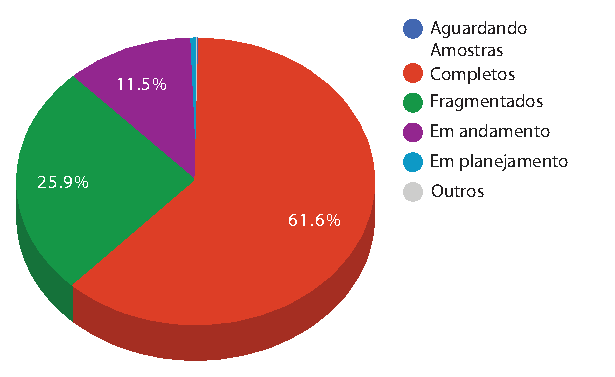
\includegraphics[width=.6\textwidth]{gold_bacterial_sequencing_status.eps} \\
	\begin{small}\textbf{Fonte: \citeonline{mukherjee2016}}\end{small}
\end{grafico}

\lipsum[2-3]

\chapter{Implementação}
\label{cap:implementacao}

\section{Algoritmo}

\begin{algorithm}[H]
   \SetAlgoLined
   \Entrada{$S,\eta, U$} 
   \Saida{Número esperado de nodos atingidos}
   \Inicio{
   $\sigma(S) = 0$ \\
    \Para{cada $u \in S$}{
   $\sigma(S)\leftarrow \sigma(S)+\textsc{Backtrack}(u,\eta,W,U)$\\
     }
   }
   \Retorna{$\sigma(S)$}
   \label{alg1}
   \caption{\textsc{Esperança}}
 \end{algorithm}

% ----------------------------------------------------------
% Resultados e Discussão
% ----------------------------------------------------------
\chapter{Resultados}
\label{cap:resultados}

\begin{table}[!htb]
\centering
\caption{Informações de montagem dos genomas de referência}
\label{tab:informacoes_montagem}
\begin{tabular}{cccc}
\toprule
\textbf{Organismo} & \textbf{Montador} & \textbf{Bases com N} & \textbf{\textit{Scaffolds}} \\ \midrule
\rowcolor[HTML]{F3F3F3} 
\textbf{\textit{Corynebacterium pseudotuberculosis 262}} & & & \\
\rowcolor[HTML]{DBDEDE} 
 & \textit{SPADES} & 2893857 & 4611 \\
\rowcolor[HTML]{F3F3F3} 
\textbf{\textit{Staphylococcus aureus A--S391\_USA300}} & & & \\
\rowcolor[HTML]{DBDEDE} 
 & \textit{ABySS} & 3893185 & 5012 \\
\rowcolor[HTML]{F3F3F3} 
 & \textit{ABySS2} & 3821622 & 125 \\
\rowcolor[HTML]{DBDEDE} 
 & \textit{Allpaths-LG} & 2880676 & 19 \\
\rowcolor[HTML]{F3F3F3} 
 & \textit{Bambus2} & 2862930 & 17 \\
\rowcolor[HTML]{DBDEDE} 
 & MSR-CA & 2872905 & 17 \\
\rowcolor[HTML]{F3F3F3} 
 & SGA & 3128388 & 546 \\
\rowcolor[HTML]{DBDEDE} 
 & \textit{SOAPdenovo} & 2924135 & 175 \\
\rowcolor[HTML]{F3F3F3} 
 & \textit{Velvet} & 2877995 & 173 \\
\rowcolor[HTML]{DBDEDE} 
\textbf{\textit{Rhodobacter sphaeroides 2.4.1}} & & & \\
\rowcolor[HTML]{F3F3F3} 
 & \textit{ABySS} & 5160167 & 2714 \\
\rowcolor[HTML]{DBDEDE} 
 & \textit{ABySS2} & 5331930 & 480 \\
\rowcolor[HTML]{F3F3F3} 
 & \textit{Allpaths-LG} & 4609785 & 38 \\
\rowcolor[HTML]{DBDEDE} 
 & \textit{Bambus2} & 4428612 & 92 \\
\rowcolor[HTML]{F3F3F3} 
 & \textit{CABOG} & 4259679 & 130 \\
\rowcolor[HTML]{DBDEDE} 
 & MSR-CA & 4498559 & 44 \\
\rowcolor[HTML]{F3F3F3} 
 & SGA & 5614693 & 2096 \\
\rowcolor[HTML]{DBDEDE} 
 & \textit{SOAPdenovo} & 4627058 & 312 \\
\rowcolor[HTML]{F3F3F3} 
 & \textit{Velvet} & 4615068 & 382 \\ \bottomrule \\
\end{tabular}
\begin{small}\textbf{Fonte: \citeonline{gapblaster2016}}\end{small}
\end{table}

\begin{quadro}[!htb]
	\centering
	\caption{Comparação das funcionalidades do \textit{GapBlaster}, \textit{FGAP} e \textit{GapFiller}}
	\label{quadro:comparacao_funcionalidades}
	\resizebox{\textwidth}{!}{\begin{tabular}{lccc}
			\toprule
			\multicolumn{1}{c}{\textbf{Funcionalidades}} & \textbf{\textit{GapBlaster}} & \textbf{\textit{FGAP}} & \textbf{\textit{GapFiller}} \\ \midrule
			\rowcolor[HTML]{F3F3F3} 
			Método de alinhamento & \textit{Legacy Blast}, \textit{Blast+} ou \textit{MUMmer} & \textit{Blast+} & \textit{Bowtie} ou BWA \\
			\rowcolor[HTML]{DBDEDE} 
			Ajuste do tamanho da região flanqueadora & Sim & Sim & Sim \\
			\rowcolor[HTML]{F3F3F3} 
			Permite curadoria manual & Sim & Não & Não \\
			\rowcolor[HTML]{DBDEDE} 
			Realiza análise automática & Sim & Sim & Sim \\
			\rowcolor[HTML]{F3F3F3} 
			Usa leituras pareadas para fechar \textit{gaps} & Não & Não & Sim \\
			\rowcolor[HTML]{DBDEDE} 
			Usa \textit{contigs} para fechar \textit{gaps} & Sim & Sim & Não \\
			\rowcolor[HTML]{F3F3F3} 
			Lê arquivos nos formatos FASTQ, SAM e BAM & Não & Não & Sim \\
			\rowcolor[HTML]{DBDEDE} 
			Executa código em paralelo & Não & Sim & Não \\
			\rowcolor[HTML]{F3F3F3} 
			Interface gráfica & Sim & Não & Não \\
			\rowcolor[HTML]{DBDEDE} 
			Melhora o resultado de outros programas & Sim & Não foi testado & Não foi testado \\
			\rowcolor[HTML]{F3F3F3} 
			Fecha \textit{gaps} corretamente & Sim & Sim & Sim \\ \bottomrule \\
	\end{tabular}}
	\begin{small}\textbf{Fonte: \citeonline{gapblaster2016}}\end{small}
\end{quadro}

% ----------------------------------------------------------
% Considerações Finais
% ----------------------------------------------------------
\chapter{Conclusão}
\label{conclusao}

\lipsum[31-33]

% ----------------------------------------------------------
% ELEMENTOS PÓS-TEXTUAIS
% ----------------------------------------------------------
\postextual
% ----------------------------------------------------------

% ----------------------------------------------------------
% Referências bibliográficas
% ----------------------------------------------------------
\bibliography{bibliografia}
% ---


% ----------------------------------------------------------
% Apêndices
% ----------------------------------------------------------

% ---
% Inicia os apêndices
% ---
\begin{apendicesenv}
	
	% Imprime uma página indicando o início dos apêndices
	\partapendices
	
% ----------------------------------------------------------
\chapter{Quisque libero justo}
% ----------------------------------------------------------

\lipsum[50]

% ----------------------------------------------------------
\chapter{Nullam elementum urna}
% ----------------------------------------------------------
\lipsum[55-57]
	
\end{apendicesenv}
% ---

% ----------------------------------------------------------
% Anexos
% ----------------------------------------------------------

% ---
% Inicia os anexos
% ---
\begin{anexosenv}
	
	% Imprime uma página indicando o início dos anexos
	\partanexos
	
	% ---
    \chapter{Morbi ultrices rutrum lorem}
    % ---
    \lipsum[30]

    % ---
    \chapter{Cras non urna sed}
    % ---

    \lipsum[31]

    % ---
    \chapter{Fusce facilisis lacinia dui}
    % ---

    \lipsum[32]
	
\end{anexosenv}

\end{document}
